\section{Experiments on synthetic data\label{section:evaluation-experiments-on-synthetic-data}}

The QSM and ASM algorithms are evaluated here on synthetic data. The aim is to study their performance when the problem size, in terms of number of states of the target model, grows significantly beyond those of the case-studies presented in Section~\ref{section:evaluation-experiments-on-case-studies}. In this particular setting, we do not rely on additional domain knowledge such as fluents, goals or models of legacy components.

Section~\ref{subsection:evaluation-abbadingo} describes the methodology used to generate automata, learning and test samples. Section~\ref{classification:gain} discusses the gain in terms of generalization accuracy of the QSM algorithm with respect to the original RPNI or Blue-Fringe algorithms. The number of generated queries by QSM is reported in section~\ref{number:queries}. Section~\ref{cpu:time} gives comparative performances in terms of induction CPU time.

\subsection{Evaluation protocol\label{subsection:evaluation-synthetic-protocol}}

The procedure that has been used to evaluate ASM and QSM on synthetic data is inspired from the Abbadingo protocol \cite{Lang:1998}. Roughly, evaluating an induction algorithm with this protocol consists in running it on learning samples of increasing size, in terms of their number of positive and negative strings. The accuracy of the induced model is measured in terms of the number of strings of a test sample that the learned model correctly classifies. This is made clearer below.

Experiments here are made on random LTS of increasing sizes: $n$ = 20, 50, 100 and 200 states. As in Abbadingo, only alphabets of two symbols are considered (see Chapter \ref{chapter:stamina} about the influence of the alphabet size on evaluation of induction algorithms). The randomly generated automata are trimmed to remove unreachable states and minimized to obtain canonical target machines. Moreover, only automata without sink state are kept for the experiments. Such states typically capture deadlocks in multi-agent systems considered in our context and should always be avoided. The number of states of an automaton generated using this procedure is approximately 3/5 of the requested size. The latter has been increased accordingly.

For a given target LTS, an initial sample of $n^2$ different strings has been first synthesized. These strings are randomly generated without replacement using a uniform distribution over the collection of all binary strings of length $[0, p+5]$ where $p$ is the depth of the automaton. The depth of an automaton is defined as the length of the the longest shortest path from the initial state to any other state. This bound is chosen so as to ensure that deepest states have a good change to be reached by at least one input string of a sample, a necessary condition for structural completeness of the sample (see Section \ref{section:inductive-background}). The procedure is such that the sample contain positive and negative strings in roughly equal proportion.
 
A maximal sample size of $\frac{n^2}{2}$ strings was experimentally observed as offering the convergence for all tested algorithms. The learning experiments are launched on increasing proportions of this nominal training sample, i.e. 3\%, 6\%, 12.5\%, 25\%, 50\% and 100\%.

Test samples of at most $\frac{n^2}{2}$ strings are used to measure the generalization accuracy of the learned model. The accuracy measure is precisely reported as the percentage of the test strings correctly classified by the learned model.

Training and test samples are guaranteed not to overlap. Moreover, in the case of the QSM algorithm, test samples do not contain the additional strings which were submitted to the oracle during the interactive learning phase.

All experiments reported hereafter have been performed on at least 10 randomly generated automata for each size and 5 randomly generated samples for each of them.

\subsection{Synthetic evaluation of QSM}

This section reports evaluation results for the QSM algorithm. An automatic oracle has been implemented to answer the questions asked during its execution. This oracle correctly answers the membership queries since it has access to the target LTS.

\subsubsection*{Generalization accuracy}

Figure~\ref{image:evaluation-qsm-accuracy} reports, for several target sizes, the proportion of independent test samples correctly classified while increasing the learning sample size. Comparative performances are given for RPNI, Blue-fringe, QSM-rpni (QSM with the RPNI merging order) and QSM-fringe (QSM with the Blue-fringe strategy).

\begin{figure}
\centering
\scalebox{.25}{
  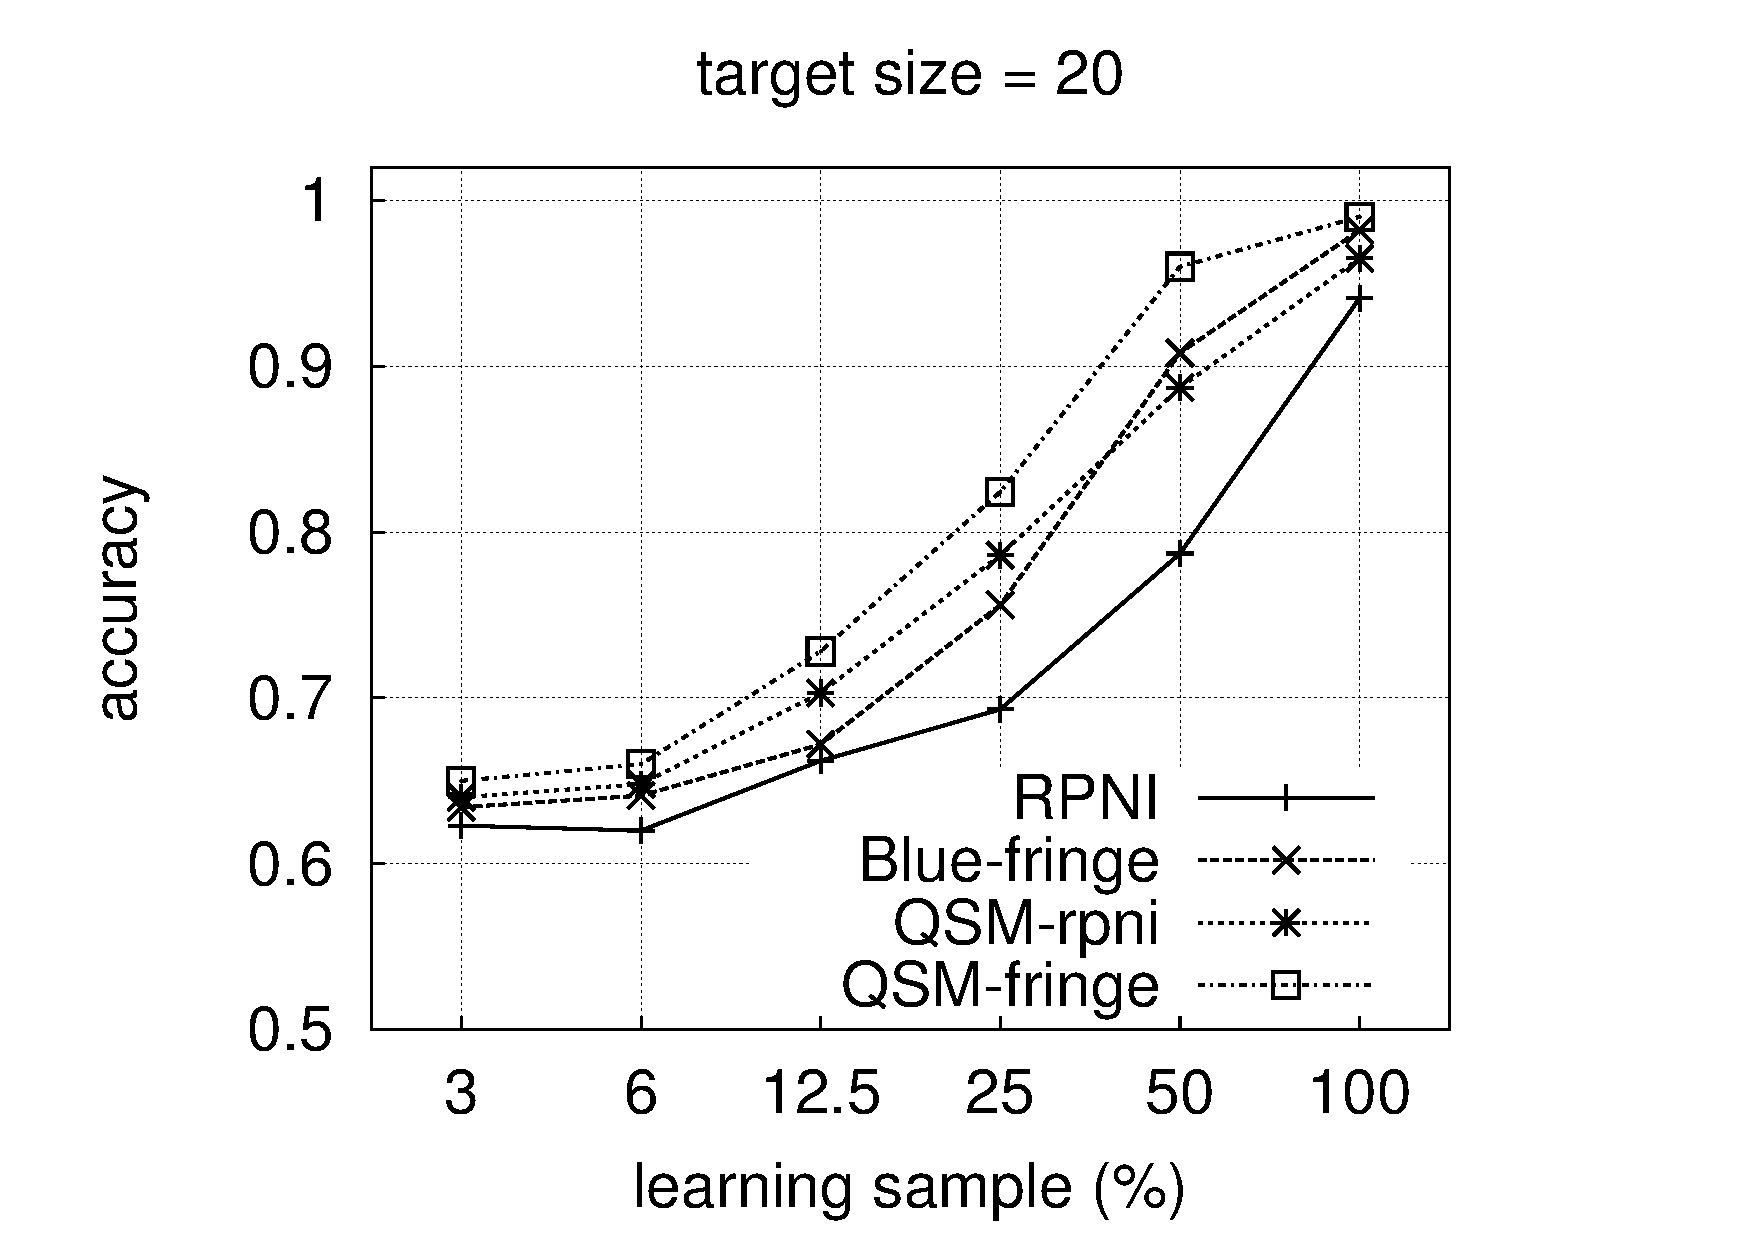
\includegraphics[trim=0mm  21mm 45mm 0mm, clip, page=1]{src/5-evaluation/images/accuracy}
  \includegraphics[trim=30mm 21mm 35mm 0mm, clip, page=2]{src/5-evaluation/images/accuracy}
}\vspace{0.35cm}
\scalebox{.25}{
  \includegraphics[trim=0mm  0mm 45mm 0mm, clip, page=3]{src/5-evaluation/images/accuracy}
  \includegraphics[trim=30mm 0mm 35mm 0mm, clip, page=4]{src/5-evaluation/images/accuracy}
}
\caption{Classification accuracy of QSM\label{image:evaluation-qsm-accuracy}.}
\end{figure}

Results from Section \ref{subsection:evaluation-bluefringe-on-casestudies} on case-studies are confirmed here since Blue-fringe outperforms RPNI for sparse training samples. Moreover, significant improvements of the generalization accuracy is observed thanks to the interactive feature. The QSM algorithm outperforms the original RPNI and Blue-fringe systematically. Interestingly, QSM-rpni also overcomes the original Blue-fringe algorithm. When the classification rate of test samples reached 100\%, the proposed solutions were always isomorphic to the target machines.

The relative performances described above do not depend much of the target size. It should be noted that the learning sample sizes are well chosen to illustrate the convergence of the standard RPNI and Blue-fringe algorithms. When the target size grows (especially for $n=200$) the QSM-fringe has already nearly converged with only 1.5\% of the nominal learning sample size. Such a gain can also be explained by the role played by the oracle. The QSM algorithm tends to elicit a characteristic sample by submitting queries to the user. This issue is further investigated in section~\ref{subsection:evaluation-synthetic-queries-on-qsm} where the number of queries is reported as function of the learning sample size.

\subsubsection*{Number of queries\label{subsection:evaluation-synthetic-queries-on-qsm}}

An important aspect of QSM is the number of queries submitted to the oracle. When the oracle is an end-user, as in the RE context, this factor indeed drives the usability of the approach in practice. 

Figure~\ref{image:evaluation-qsm-number-of-questions} presents the number of generated queries depending on the learning sample size, for several target sizes. Results are given for QSM-rpni and QSM-fringe. In each case, the number of generated strings which are classified by the oracle either as positive or negative are reported separately.

The number of strings classified as positive tends to increase initially with the learning sample size before staying roughly constant when the learning process has nearly converged. The additional information required to guarantee correct identification mostly depends on the negative strings.

Figure~\ref{image:evaluation-qsm-number-of-questions} shows that QSM-fringe tends to generate fewer strings classified as
negative by the oracle as compared to QSM-rpni. The figure also shows that the number of negative strings decreases with the learning sample size. In other words, the number of strings classified as negative decreases while the algorithm converges. This illustrates that the generalization obtained while merging states is more sound when performed with more data.

\begin{figure}
\centering
\scalebox{.25}{
  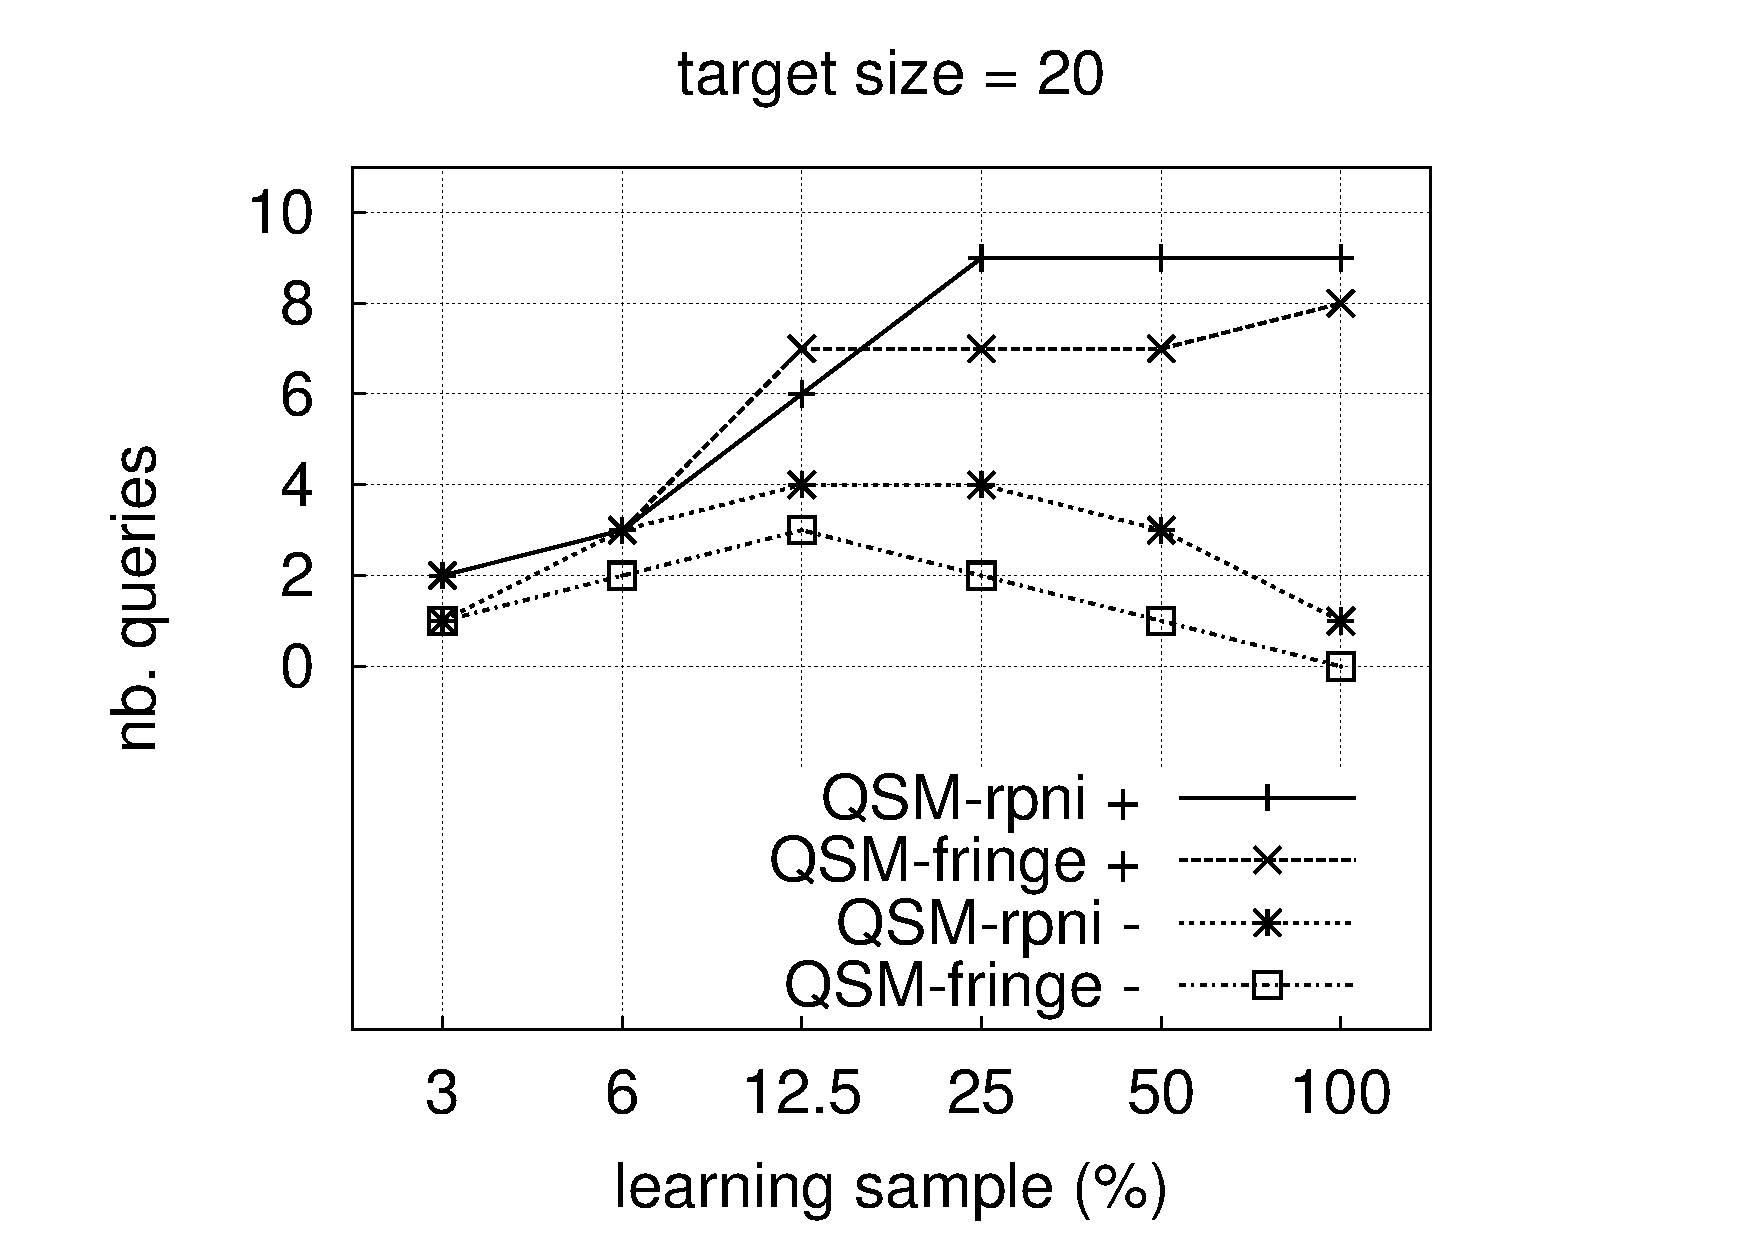
\includegraphics[trim=0mm  21mm 45mm 0mm, clip, page=1]{src/5-evaluation/images/queries}
  \includegraphics[trim=30mm 21mm 35mm 0mm, clip, page=2]{src/5-evaluation/images/queries}
}\vspace{0.35cm}
\scalebox{.25}{
  \includegraphics[trim=0mm  0mm 45mm 0mm, clip, page=3]{src/5-evaluation/images/queries}
  \includegraphics[trim=30mm 0mm 35mm 0mm, clip, page=4]{src/5-evaluation/images/queries}
}
\caption{Number of queries generated by QSM\label{image:evaluation-qsm-number-of-questions}.}
\end{figure}

\subsubsection*{Induction time\label{cpu:time}}

Figure~\ref{image:evaluation-qsm-time} reports the induction time while varying learning sample size and target size. All tests were executed with Java 5.0 on a Pentium-IV 3 GHz computer with 1Gb of RAM. 

The RPNI, Blue-fringe and QSM algorithms go through different phases according to the amount of available data:
\begin{itemize} 
\item Initially, the CPU time tends to increase with the learning sample size. In this first phase, the learning time follows the increase of the sample size. 
\item When the learning sample becomes richer, better generalizations can be obtained by merging states in a more sound way. A comparison between curves in Fig.~\ref{image:evaluation-qsm-accuracy} and in Fig.~\ref{image:evaluation-qsm-time} shows that the classification rates of new data increases while the learning time reaches its maximum. 
\item The last phase is observed when the algorithm rapidly converges to a good model. Classification accuracy tends to 100\% and the CPU time is decreased because the right merging operations are performed directly. 
\end{itemize}

\begin{figure}
\centering
\scalebox{.25}{
  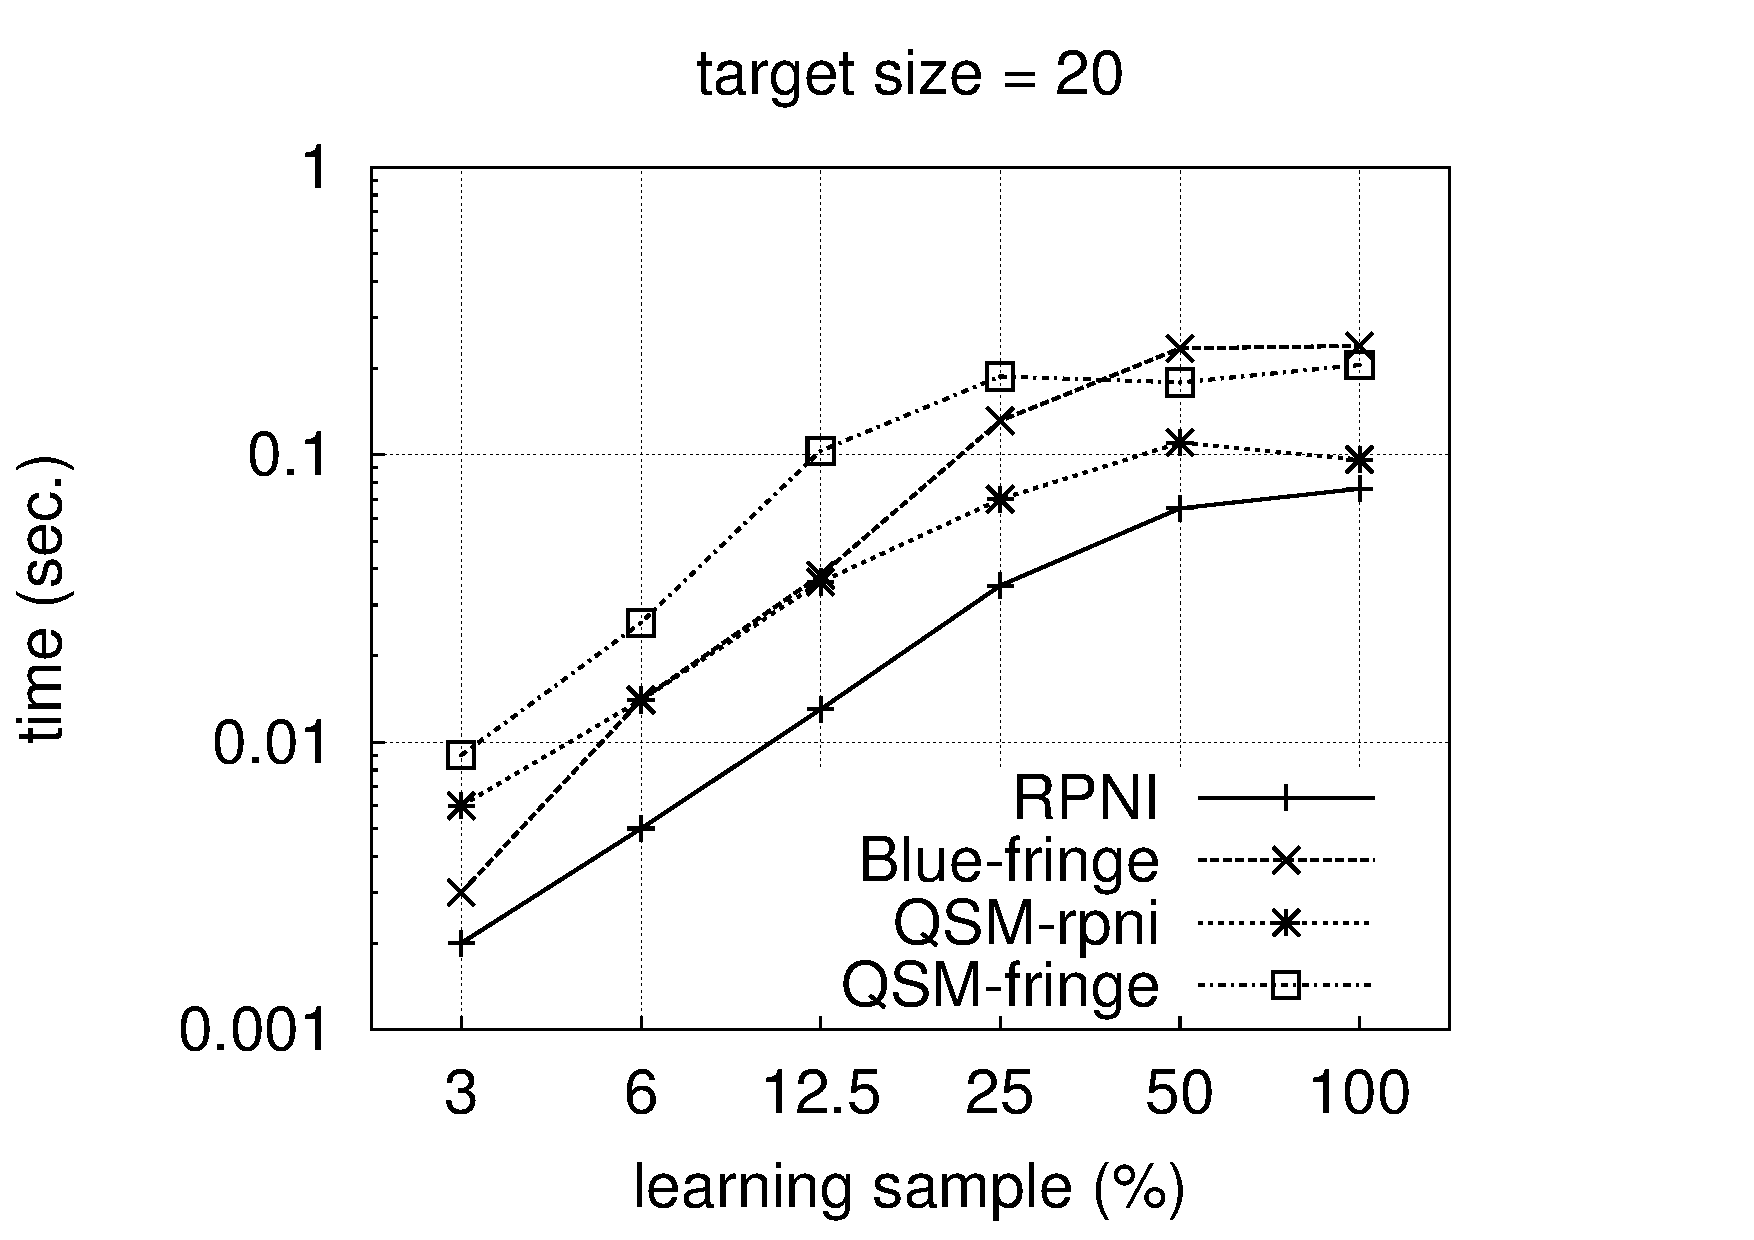
\includegraphics[trim=0mm  21mm 45mm 0mm, clip, page=1]{src/5-evaluation/images/time}
  \includegraphics[trim=30mm 21mm 35mm 0mm, clip, page=2]{src/5-evaluation/images/time}
}\vspace{0.35cm}
\scalebox{.25}{
  \includegraphics[trim=0mm  0mm 45mm 0mm, clip, page=3]{src/5-evaluation/images/time}
  \includegraphics[trim=30mm 0mm 35mm 0mm, clip, page=4]{src/5-evaluation/images/time}
}
\caption{Induction time with QSM\label{image:evaluation-qsm-time}.}
\end{figure}

Known tendencies of induction algorithms of the RPNI family are confirmed in our experiments (see, e.g., \cite{Lang:1998}). However, the curves of QSM are shifted left with respect to the learning sample size. As already observed in Fig.~\ref{image:evaluation-qsm-accuracy} convergence is indeed faster for the QSM algorithm. The relative time performance of the QSM algorithm with respect to RPNI or Blue-fringe depends on two contradictory effects:
\begin{itemize}
\item On the one hand, whenever a string is classified as negative by the oracle, QSM is called recursively on an extended sample. Each new call increases the CPU time as it could be considered as a new run of the RPNI or Blue-fringe algorithm. This run can however be interrupted and replaced by another one if a new negative example is included after an additional query.
\item On the other hand, due to its faster convergence, QSM can obtain better results with fewer data originally provided. 
\end{itemize}
 
The CPU times should thus be compared while considering the relative classification results of the various approaches. For instance, when the target size is 200 and 3\% of the full training sample is used, QSM-fringe runs an order of magnitude slower than Blue-fringe. However, the classification accuracy of QSM-fringe is 95\% while it is 67\% for Blue-fringe for the same amount of data. When the training size increases QSM-fringe actually becomes slightly faster than Blue-fringe because it has already nearly converged to the optimal solution.

\subsection{Synthetic evaluation of ASM}

As discussed in Section \ref{section:inductive-from-hMSC}, ASM reduces to RPNI when its input is a PTA instead of an arbitrary DFA. As in Section \ref{subsection:evaluation-casestudies-asm} when evaluated on case studies, the objective of the evaluation here is mostly to quantify the proportion of domain-specific control information required to get better generalization results. 

The experimentation protocol that we used to achieve this objective is a slight adaptation of the one discussed in Section \ref{subsection:evaluation-synthetic-protocol}:
\begin{itemize}

\item Experiments here are made on randomly generated target LTS with 32 and 64 states. As previously, we restricted our attention to alphabets of 2 symbols.

\item Learning and test samples are randomly generated in a similar way as before. However, a specific procedure has been set up to simulate the control information typically offered by a hMSC:
\begin{itemize}

\item Unique labels have been associated to randomly chosen states of the target LTS. Increasing proportions of the number of states labeled in this way have been used: 5\%, 10\%, 20\% and 100\%.

\item For a given learning sample, an augmented $PTA$ is then been built. used by ASM are labeled by jointly visiting it with the target DFA and reporting encountered labels.
\end{itemize}
\end{itemize}
 
Figure~\ref{fig:expe:accuracy} reports the proportion of independent test samples correctly classified while increasing the learning sample. Curves in this plots correspond to executions of RPNI, Blue-Fringe and MSM with different labeling proportions. Each point in these plots is the average value computed over 200 independent runs. MSM overcomes RPNI on all executions, which was actually expected, but illustrates experimentally that forcing to merge initially some (correctly labeled!) states does not prevent from converging. 5\% of labeling information is comparable, from the point of view of the generalization accuracy, to the use of the Blue-Fringe heuristic for selecting state pairs to be merged. Beyond this proportion, the accuracy continues to increase. Interestingly, it is already visible when the sample is sparse. This fact is particularly helpful in our RE context, where learning sample is initially provided by an end-user.
Moreover, it is worth noting that, as pointed out in section~\ref{mustmerge}, the identification of the target does not reduce to a trivial problem even with 100\% of labeling information when only few negative examples are available. 

%\begin{figure}[H]
%\begin{center}
%\scalebox{.21}{\includegraphics*{expe_accuracy.jpg}}
%\caption{Classification accuracy for RPNI, Blue-Fringe and MSM\label{fig:expe:accuracy}.}
%\end{center}
%\vspace*{-.75cm}
%\end{figure}

Although not yet implemented, we are confident that using mandatory merge constraints would also improve the generalization accuracy  of the Blue-Fringe and QSM algorithms (the interested reader may refer to~\cite{Dupont08} for an experimental comparison between RPNI, Blue-Fringe and QSM without labeling constraints).




